\begin{frame}
    \frametitle{Data Analysis}
    \begin{columns}[T] % Top alignment for each column
        \begin{column}{.48\textwidth} % Left column
            \begin{itemize}
                \item \textbf{Packet Delivery Rates:}
                \begin{itemize}
                    \item With ACKs: 100\% success.
                    \item Without ACKs: 89.24\% success.
                \end{itemize}
                \item \textbf{Communication Overhead:}
                \begin{itemize}
                    \item Additional 110 messages retransmitted with ACKs.
                    \item Total messages: 1144.
                \end{itemize}
                \item \textbf{Energy Consumption:}
                \begin{itemize}
                    \item Higher energy expenditure due to ACKs.
                    \item Important in energy-constrained environments.
                \end{itemize}
                \item \textbf{Future Optimizations:}
                \begin{itemize}
                    \item Explore adaptive ACK strategies.
                    \item Balance reliability with energy usage.
                \end{itemize}
            \end{itemize}
        \end{column}
        \begin{column}{.48\textwidth} % Right column
            \begin{figure}
                \centering
                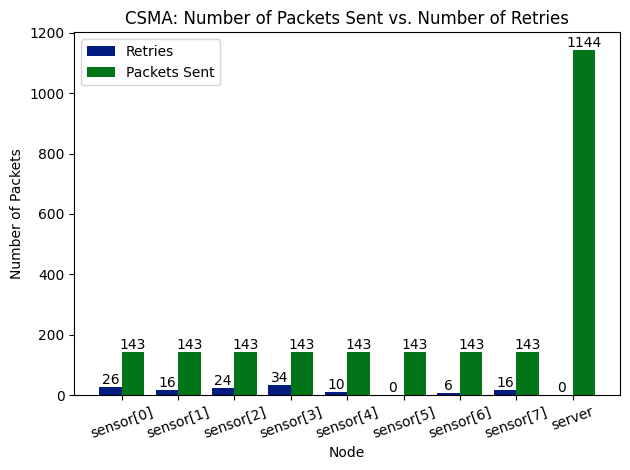
\includegraphics[width=\linewidth]{images/ack.png}
                \label{fig:ack}
                \vspace{-1.25cm}
            \end{figure}
            \begin{figure}
                \centering
                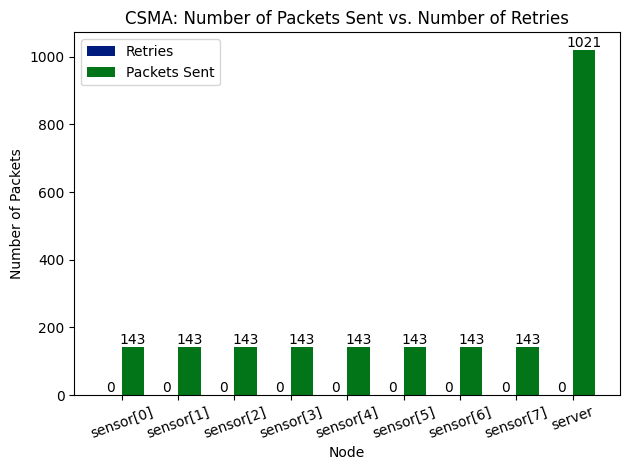
\includegraphics[width=\linewidth]{images/noack.png}
                \label{fig:noack}
            \end{figure}
        \end{column}
    \end{columns}
\end{frame}

